
\begin{frame}{Ziel}{\src{simple-device.c}}
 \begin{itemize}
  \item Verbindung {\em userspace}-{\em userspace}
  \begin{itemize}
   \item alles ist ein File
  \end{itemize}
  \item {\em devicefile} 
  \begin{itemize}
   \item \cod{mknod {\em device-file} {\em type} major minor}
  \end{itemize}
  \item die elementaren Operationen
 \end{itemize}
\end{frame}


\subsection{userspace: alles ist ein File}
\begin{frame}{Alles ist ein File}{etwas genauer}
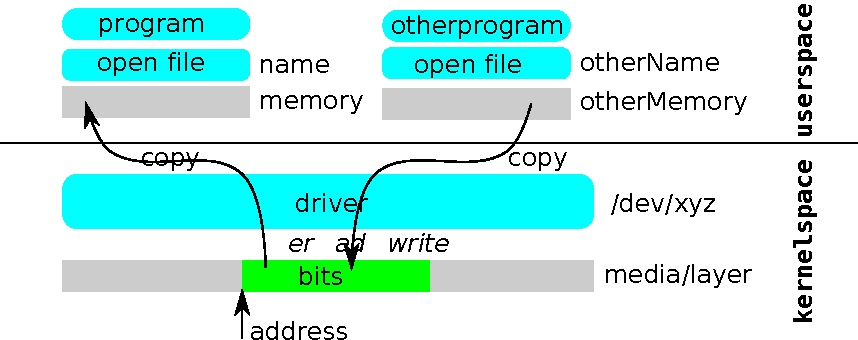
\includegraphics[width=0.875\textwidth]{driver-file.pdf}
%\includesvg{driver-file}
\end{frame}

\begin{frame}{\src{simple-device.c}:im alles ist ein File}
             {Die elementaren Operationen im {\em userspace}}
 \vspace{-4mm}
  \begin{itemize}
   \item \cod{open}
   \item \cod{read}
   \item \cod{write}
   \item \cod{close}
  \end{itemize}
\end{frame}

\begin{frame}{Die elementaren Operationen im {\em userspace}}
             {der Befehl \cod{cat}}
  \begin{itemize}
   \item \cod{cat {\bf device}}
   \begin{itemize}
    \item \cod{open},\cod{read},\cod{close}
   \end{itemize}
   \item \cod{cat file > {\bf device}}
   \begin{itemize}
    \item \cod{open},\cod{write},\cod{close}
   \end{itemize}
  \end{itemize}
\end{frame}

\begin{frame}{Der Devicefile \cod{device}}
 \begin{itemize}
  \item ist ein File
  \item bezeichnet ein {\em device}
  \item ist normalerweise im Verzeichnis \cod{dev}
  \begin{itemize}
   \item muss aber nicht 
  \end{itemize}
 \end{itemize}
 \begin{block}{Beispiele}
  \begin{itemize}
   \item \cod{/dev/ttyUSB0} die serielle Schnittstelle
   \item \cod{/dev/mmcblk0} die SD-Karte auf \target
   \item \cod{/dev/random}, \cod{/dev/urandom}
   \item ...
  \end{itemize}
 \end{block}
\end{frame}

%\begin{frame}{Beispiele}{alles ist ein File}
%{\cod{/dev/random}, 
%\cod{/dev/urandom}, \cod{/dev/sda}}
% \begin{itemize}
%  \item \cod{cat /dev/random | hexdump -C} 
%  \begin{itemize}
%    \item sammelt das Rauschen: langsam
%   \end{itemize}
%  \item \cod{dd if=/dev/sda count=1 | hexdump -C}
%  \begin{itemize} 
%    \item der MBR 
%  \end{itemize}  
% \end{itemize}
%\end{frame}

\begin{frame}[fragile]{Die Verbindung {\em file - device}}{Devicefile}
\begin{block}{Beispiel: \cod{/dev/ttyUSB0}\footnote{gemacht mit \cod{ls -l}}}
\vspace{-5mm}
{\footnotesize
\begin{verbatim}
crw-rw---- 1 root uucp   188,  0 11. Nov  20:27 /dev/ttyUSB0
|            |    |      |     |                |
|            |    |      |     |                name
|            |    |      |     minor                
|            |    |      major 
|            |    group 
|            owner
devicetyoe
\end{verbatim}
}
\end{block}
\vspace{-6mm}
\begin{block}{für uns wichtig:}
 \vspace{-3mm}
 \begin{description}
  \item[major] Code für die {\em device} Klasse
  \item[minor] Nummer für ein {\em device} 
 \end{description}
\end{block}
\end{frame}

\begin{frame}{Major:Minor}{objektorientierte Interpretation}
 \begin{description}
  \item[major] Code für die {\Large Klasse}
  \item[major] Code für die {\Large Instanz}
 \end{description}
\end{frame}

\begin{frame}[fragile]{Der Befehl \cod{mknod}}{erzeugt einen {\em Devicefile}}
\begin{verbatim}
Usage: mknod [-m MODE] NAME TYPE MAJOR MINOR                                    
                                                                                
Create a special file (block, character, or pipe)                               
                                                                                
        -m MODE Creation mode (default a=rw)                                    
TYPE:                                                                           
        b       Block device                                                    
        c or u  Character device                                                
        p       Named pipe (MAJOR and MINOR are ignored)                        
\end{verbatim} 
\end{frame}

\subsection{kernelspace}
\begin{frame}[fragile]{\cod{register\_chrdev}}
 \begin{itemize}
  \item erzeugt {\em major}
  \item \cod{file\_operations fops} die Fileoperationen
  \begin{itemize}
   \item call-backs
   \item siehe \cod{linux/fs.h}
  \end{itemize}
 \end{itemize}
 \begin{block}{à la \CPP}
 \begin{lstlisting}
  class File
  {
   protected:
    virtual int open(...)=0;
    virtual int flush(...)=0;
    virtual int read(...)=0;
    virtual int write(...)=0;
    ...
  };
 \end{lstlisting}
 \end{block}
 
\end{frame}

\begin{frame}{Transfer userspace $\leftrightarrow$ kernelspace}
{\cod{simple-read} und \cod{simple-write}}
\begin{center}
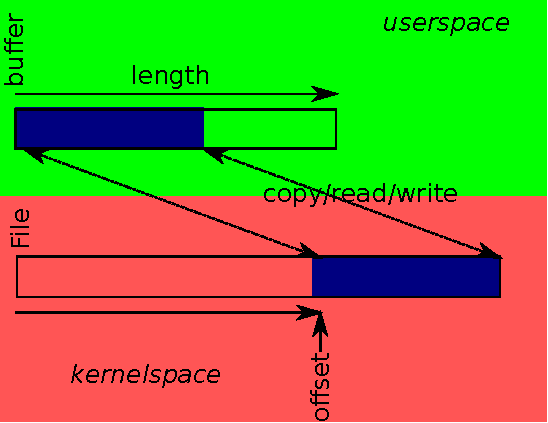
\includegraphics[height=0.75\textheight]{user-kernel-space-copy.pdf}
\end{center}
\end{frame}


\subsection{Test}
\begin{frame}{Test}
 \begin{itemize}
  \item \cod{insmod simple-device.ko}
  \begin{itemize}
   \item $\to major$
  \end{itemize}
  \item \cod{mknod devi c {\em major} {\em i}}
  \begin{itemize}
   \item Devicefile beliebige minor
  \end{itemize}
  \item \cod{cat devi}
  \begin{itemize}
   \item lese von \cod{devi}
  \end{itemize}
  \item \cod{echo "{}hello"{} > devi}
  \begin{itemize}
   \item schreibe auf \cod{devi}
  \end{itemize}
 \end{itemize}
 \remark{\cod{devi} in \cod{/work}}
\end{frame}

\subsection{Aufgaben}
\begin{frame}{Aufgaben}
\begin{itemize}
 \item \cod{src/simple-device.c} für \host/\targetS
 \item Registrierung/Deregistrierung  in \cod{sys/class}
 \begin{itemize}
  \item  \cod{class\_create}
  \item  \cod{device\_create}
 \end{itemize}
\end{itemize}
\end{frame}


%\begin{frame}{simple-device}{userspace$\leftrightarrow$kernelspace}
% \begin{itemize}
%  \item alles ist ein File
%  \begin{itemize}
%   \item {\em stream of bits}
%  \end{itemize}
%  \item Trennung {\bf userspace} {\bf kernelspace}
%  \begin{itemize}
%   \item meltdown, spectre
%  \end{itemize}
% \end{itemize}
%\end{frame}
%
%\begin{frame}{simple-device}
% \begin{description}
%  \item[Module] \cod{src/simple-device.c}, \cod{src/Makefile}
%  \item[Test] 
%     \begin{itemize}
%       \item \cod{insmod simple-device.ko} Major Number
%       \item \cod{mknod -ma=rw simple c Major 1} Device File Zugriff für alle
%       \item \cod{cat simple} read 
%       \item \cod{cat aFile > simple} write
%     \end{itemize} 
% \end{description}
% \begin{todos}
%  \item Automatische Erzeugung von \cod{simple}
%  \item die \cod{file\_operations}: \cod{open} und \cod{close}
% \end{todos}
%\end{frame}
%
%\begin{frame}{\cod{simple-device.c}}{userspace $\leftrightarrow$ kernelspace}
% \begin{description}[kernelspace $\to$ userspace]
%  \item[Module] brauche  \cod{print\_hex\_dump} eine praktische Funktion
%  \item[userspace $\to$ kernelspace] \cod{simple\_write}
%  \item[kernelspace $\to$ userspace] \cod{simple\_read}
%  \item[Test] \cod{simple-device} im userspace
% \end{description}
% \todo{Erzeuge Absturz}
%\end{frame}

\begin{frame}{Problem}
\begin{itemize}
 \item Funktioniert für \host
 \item Funktioniert {\Huge nicht} für \targetS
\end{itemize}
\end{frame}
